%!TEX root = ../../main.tex
\chapter{Nutzerzentrierte Umfrage}
\label{chapter:4}

Während dieser Studienarbeit steht die Verbesserung und Restrukturierung der CO2-Runter Webseite im Vordergrund.
Dabei soll besonders auf die Nutzergruppe eingegangen werden, um mit dem bereits vorgestellten Prinzip des nutzerzentrierten Designs die Webseite für den Endnutzer ansprechender und interessanter zu gestalten.
Durch dieses Vorgehen soll die Webseite sowohl in den Punkten Design und Nutzerfreundlichkeit, als auch im Allgemeinen verbessert werden.
Das Ziel dahinter ist, dass mehr potenzielle NutzerInnen gefunden und angesprochen werden, um so zu einem klimabewussteren Denken anzuregen.

Da der/die NutzerIn im Zentrum des Vorgehens steht, werden selbstverständlich Ideen, Kritik und Einflüsse von potenziellen NutzerInnen der Webseite, aber auch von Menschen im Allgemeinen, über die bisherige Webseite benötigt.
Um diese Kritik und Einflüsse zu sammeln wird im Rahmen dieser Studienarbeit eine nutzerzentrierte Umfrage durchgeführt.
Mithilfe der Umfrage sollen Meinungen, Kritik und Ideen von unparteiischen Personen gesammelt werden, sodass diese im Anschluss ausgewertet werden können und dem Entwicklerteam entscheidende Hinweise darüber bieten, welche Aspekte der aktuellen Webseite größeren Sanierungsbedarf haben bzw.
welche Aspekte bereits ihren Zweck und Wert erfüllen.
In den folgenden Unterkapiteln wird das Vorgehen von der Sammlung der möglichen Fragen der Umfrage, bis hin zur Auswertung der Umfrageergebnisse dokumentiert.

\section{Methodik der Umfrage}

Die Methodik der Umfrage bildet das methodische Grundgerüst, das die systematische Erfassung und Analyse von Daten ermöglicht, um präzise Einblicke in die untersuchte Thematik zu gewinnen. In diesem Kapitel werden die spezifischen Vorgehensweisen und Verfahren detailliert erläutert, die im Rahmen der durchgeführten Umfrage angewendet wurden.
Von der Auswahl der Stichprobe über die Gestaltung des Fragebogens bis hin zur Datenerhebung und -auswertung werden die methodischen Schritte transparent dargestellt.

\subsection{Planung der Umfrage}
Zu Beginn jeder Umfrage steht die Planung der Umfrage.
Die Planung ist einer der wichtigsten, wenn nicht sogar der wichtigste, Schritt einer Umfrage, da auf Basis der in der Planung festgelegten Konzepte etc.
die finale Umfrage aufbaut und schlußendlich auch durchgeführt wird.
Dazu wird im Buch \texttt{Umfrage} beschrieben, dass jedes Forschungsprojekt grundsätzlich mit einer Planungsphase beginne.
Darin werden unter anderem die theoretische Fundierung der Forschungsfrage als auch die daraus resultierende Art der Froschung festgelegt.\cite{umfrage:2011}

Die Forschungsfrage wird am Anfang eines Forschungsprojektes bestimmt und steuert das weitere Vorgehen des Projektes. \cite{umfrage:2011}
In unserem Fall bearbeiten wir die Forschungsfragen: "Wie kann man mehr Menschen dazu motivieren, die CO2-Runter Webseite zu nutzen?"\ und "Wie kann man klimabewussteres Verhalten im Allgemeinen erzeugen?".

Mit der Forschungsfrage ergibt sich zumeist automatisch auch die Art der Forschung.
Dabei unterscheidet man im Allgemeinen grundsätzlich vier Arten von Untersuchungen:

\begin{itemize}
    \item \textbf{Explorative Untersuchung:} Untersucht man einen Bereich mit seiner Untersuchung bzw. Umfrage, in welchem bisher nur sehr wenige bzw. keine Informationen und Erkenntnisse vorliegen, so handelt es sich um eine explorative Untersuchung. Das Ziel einer explorativen Untersuchung ist es, einen ersten Überblick über den Untersuchungsbereich zu gewinnen und Grundlagenforschung durchzuführen. Häufig wird diese Art der Untersuchung als Umfragenforschungsprojekt als vorbereitende Forschung verwendet. \cite{umfrage:2011}
    \item \textbf{Deskriptive Untersuchung:} Bei einer deskriptiven Untersuchung gibt es bereits ein relativ großes Vorwissen. Das primäre Ziel ist hierbei Detailinformationen zu einem Thema zu erlangen. Zusätzlich im Zentrum des Interesses stehen hier Fragen nach der Verteilung bestimmter Merkmale und Merkmalskombinationen, aber auch nach Veränderungen z.B. im Zeitverlauf. \cite{umfrage:2011}\ Ergebnisse einer deskriptiven Untersuchung werden höufig in Tabellen präsentiert. Bekannt sind diese aus Printmedien und/oder dem Fernsehen.\cite{umfrage:2011}
    \item \textbf{hypothesentestende bzw. kausalanalytische Forschung:} Sollte man bei einer Untersuchung bereits vor der empirischen Untersuchung Vermutungen über die Ausprägung bestimmter Verteilungen angestellte werden, spricht man von einer hypothesentestenden Untersuchung.\cite{umfrage:2011}
\end{itemize}

Bei unserer Umfrage handelt es sich um eine kausale Untersuchung.
Das liegt daran, dass mit der Umfrage eine Ursache-Wirkung-Beziehung zwischen den Aspekten der Webseite und der Nutzerfreundlichkeit herauszufinden.
Durch die Sammlung der Daten, welche Aspekte der aktuellen Webseite gut oder schlecht bewertet wurden, kann man Hypothesen aufstellen, welche Elemente der Webseite zu einer positiven bzw. negativen Nutzererfahrung führen.\

Bevor die eigentliche Umfrage erstellt wurde, wurden in einem Dokument Fragen gesammelt um einen Fragenkatalog zu erstellen. Der Fragenkatalog dient zur Sammlung möglicher Fragen, damit diese nach der Sammelphase erneut überarbeitet und gewichtet werden können.
Der Fragenkatalog besteht aus insgesamt \textbf{31} Fragen.
Die Fragen wurden in einer Brainstorming-Aktion gesammelt und ohne Ordnung notiert.
Nach der Brainstorming-Aktion wurden die Fragen kategorisiert.
Dabei wurden die folgenden Kategorien erstellt und für die Einordnung der Fragen genutzt:

\begin{itemize}
    \item CO2 Fußabdruck
    \item Motiviation Nutzung
    \item Verbesserung Webseite
    \item aktueller Stand der Webseite
\end{itemize}

Im nächsten Schritt wurden die kategorisierten Fragen bewertet und nach ihrer Wichtigkeit eingeteilt.
Für die Bewertung wurden Ganzzahlen im Interval von 0 (= nicht so wichtig) bis 5 (= muss vorhanden sein) bewertet.
Alle Fragen die mit einer 5 gekennzeichnet wurden, wurden später automatisch mit in die Umfrage aufgenommen.
Von allen 31 Fragen wurden insgesamt 26 mit einer 5 gekennzeichnet und wurden somit 1:1 bzw. in einer ähnlichen Form in die Umfrage aufgenommen.
Selbstverständlich wurden während der Erstellung der Umfrage weitere Fragen hinzugefügt, da der Fragenkatalog lediglich als Orientierung und ersten roten Faden verwendet wurde.\

Nun wurde mit der eigentlichen Erstellung der Umfrage begonnen.
Die Umfrage wurde mithilfe von \href{https://docs.google.com/forms/u/0/}{Google Formulare} erstellt.
Da Google mit Google Formulare eine kostenlose Möglichkeit zum Erstellen von Umfragen mit vielen Features bietet, wurde auf diese Software bei der Erstellung der Umfrage gesetzt.\

Die Umfrage enthält insgesamt 5 Abschnitte.
Die Abschnitte sind hierbei mit Kategorien zu vergleichen, da darauf geachtet wurde, dass ähnliche Fragen innerhalb eines Abschnitts präsentiert werden.
Die Umfrage startet mit einem kleinen Einführungsabschnitt.
Darin werden die Teilnehmenden begrüßt und der Grund der Umfrage wird genauer erläutert.
Es wird ebenfalls darauf hingewiesen, dass es von Vorteil ist, die Originalwebseite aufzurufen.
Dies hat zum einen den Vorteil, dass die Teilnehmer die Webseite live erleben können.
Aber es bietet selbstverständlich auch eine erste Werbung.
Abschließend wird der Teilnehmende in diesem ersten Abschnitt darauf aufmerksam gemacht, dass die Umfrage ungefähr 30min dauern kann und diese anonym durchgeführt wird.
Es wird also weder eine Email, noch andere persönliche Daten für die Teilnahme an der Umfrage benötigt.

Der zweite Abschnitt thematisiert das vorhandene Wissen des Teilnehmers über den CO2-Fußabdruck im Allgemeinen.
Das Ziel dieses Abschnitts ist es, zu erfahren, inwieweit sich der Teilnehmende bereits mit den Themen CO2-Fußabdruck und Klimaschutz beschätigt hat.
Beispielhafte Fragen aus diesem Abschnitt sind zum Beispiel:

\begin{enumerate}
    \item Kennen Sie den Begriff CO2-Fußabdruck?
    \item Haben Sie sich schon einmal Gedanken über ihren CO2-Fußabdruck gemacht?
    \item Wie bewusst sind Sie sich im Allgemeinen über ihren CO2-Fußabdruck?
\end{enumerate}

Im Falle, dass die erste Frage mit \textit{Nein} beantwortet wurde, besteht die Möglichkeit, innerhalb der Umfrage ein zweiminütiges Erklärvideo zum Thema CO2-Fußabdruck anzuschauen.

Abschnitt drei behandelt das Thema \textit{Motivation}.
Innerhalb des Abschnitts steht die Frage im Fokus, wie man Menschen zu klimafreundlicherem Verhalten motivieren und anregen kann.
Zusätzlich soll auch ermittelt werden, was sich NutzerInnen eines CO2-Rechners von der Webseite erwarten bzw. erhoffen.
In diesem Teil der Umfrage sind zudem häufig Textfelder unter den Antwortmöglichkeiten, damit die Teilnehmer ihre eigenen Anregungen/Ideen/Meinungen zu den Themen kommunizieren können.
Ziel dieses Abschnitts ist es, herauszufinden, was die NutzerInnen und vor allem (noch) potenzielle NutzerInnen von der Webseite erwarten und fordern.
Durch das hier erhaltene Feedback kann bei der späteren Implementierung der neuen Features darauf geachtet werden, den NutzerInnen gerecht zu werden.
Der Abschnitt beinhaltet zum einen Fragen, die mit \textit{Ja} oder \textit{Nein} beantwortet werden, wie z.B.:

\begin{enumerate}
    \item Sind Sie bereits aktiv dabei, unser Klima zu schützen?
    \item Motiviert es Sie, wenn Sie ihren Fußabdruck mit anderen Nutzern vergleichen können?
    \item Würde ihnen ein Punktesystem helfen, ihren CO2-Fußabdruck häufiger zu berechnen?
\end{enumerate}
Jedoch befinden sich auch Fragen, die mehrere Auswahlmöglichkeiten bieten, um auf die Frage zu antworten.
Beispielhafte Fragen sind hier:
\begin{enumerate}
    \item Welche Anreize könnten Sie dazu motivieren, die Webseite häufiger zu verwenden?
    \item Welche Möglichkeiten müssten eine Webseite ihnen bieten, um unser Klima (noch) aktiver zu schützen?
\end{enumerate}
Dabei stehen sowohl vordefinierte Auswahlmöglichkeiten zur Verfügung, als auch ein Feld, bei welchem die Teilnehmer eigene Antwortmöglichkeiten eingeben können.
Am Ende des Abschnitts besteht für den Teilnehmer die Option, eigene Ideen einzubringen, wie klimafreundlicheres Verhalten erzeugt werden kann.

Innerhalb des nächsten Abschnitts, Abschnitt 4, wird das Thema \textit{Nutzerfreundlichkeit} behandelt.
Hier wird der Teilnehmende bezüglich der Nutzerfreundlichkeit der aktuellen Webseiten befragt.
Zudem soll ermittelt werden, wie die Nutzerfreundlichkeit und das Zurechtfinden auf der Webseite besser gewährleistet werden kann.
Das gewünschte Resultat ist hierbei, dass ein generelles Bild über die Nutzerfreundlichkeit der aktuellen CO2-Runter Webseite gewonnen wird.
Zusätzlich sollen durch das Feedback der Teilnehmenden wichtige Punkte gewonnen werden, die im späteren Designprozess der neuen CO2-Runter Webseite zum Thema Nutzerfreundlichkeit mit eingearbeitet werden können.
Die Mehrheit der Fragen des Abschnitts sind so gestaltet, dass den Teilnehmern Screenshots aus der aktuellen Webseite präsentiert werden.
Auf dem Screenshot sind die im Fokus stehenden Aspekte der Webseite mit roten Boxen hinterlegt. Abbildung \ref{fig:picture-of-screenshot-with-boxes} zeigt ein solches Beispiel:

\begin{figure}[H]
    \centering
    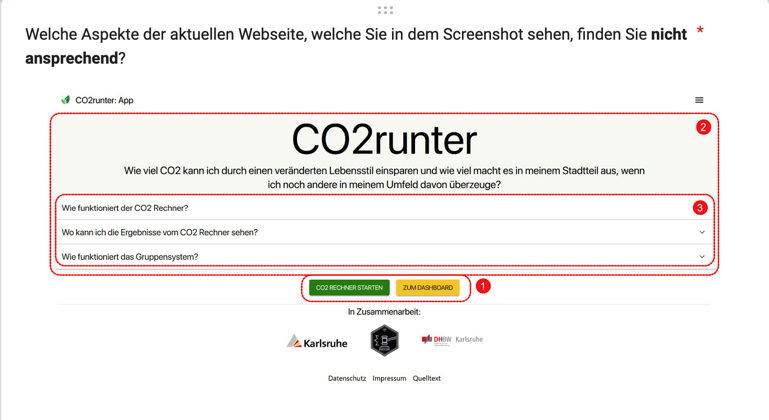
\includegraphics[width=1\textwidth]{images/05/picture_of_screenshot_with_boxes}
    \caption{Frage aus Abschnitt 4, rote Boxen zur Erkennung des Fokus}
    \label{fig:picture-of-screenshot-with-boxes}
\end{figure}

Anschließend werden dem Teilnehmenden Ankreuzmöglichkeiten anhand der Zahlenwerte geboten, um die Frage zu beantworten.
Es gibt auch jedes Mal die Antwortmöglichkeit, die alle Optionen verneint bzw. bejaht.
Sowie die Möglichkeit, eine freie Antwort in Form eines Kurztextes zu verfassen.
Da es innerhalb des CO2-Rechners der Webseite auch die Möglichkeit gibt, bei Fragen eine detaillierte Ansicht zu aktivieren, wird die Notwendigkeit und Meinung nach solch einem Feature abgefragt.
Die detaillierte Ansicht wandelt hierbei eine Frage in mehrere Unterfragen um, bei der detailliertere Fragen zu einem bestimmten Themenbereich gestellt werden.\

Der letzte Abschnitt behandelt das Thema \textit{Design}.
Dabei wird sowohl auf das aktuelle Design der CO2-Runter Webseite eingegangen, als auch auf neu erstellte Designprototypen.
Die Teilnehmenden werden aufgefordert, dass alte Design der Webseite zu bewerten.
Im Gegenzug bekommen sie auch Vorschläge zu neuen Designmöglichkeiten, die mit der Software Figma erstellt wurden.
Das Ziel des letzten Abschnitts ist es, herauszufinden, in welchen Teilen der Webseite ein verbessertes Design erwünscht ist.
Dadurch soll gleichzeitig auch die Nutzerfreundlichkeit und die allgemeine Nachfrage nach der CO2-Runter Webseite steigen.
Es gibt dabei zwei grundsätzliche Fragetypen innerhalb des Abschnitts: Bewertungsfragen und Ja/Nein/Neutral-Fragen.
Bei den Bewertungsfragen wird dem Teilnehmenden ein Screenshot des relevanten Themas/Bereichs gezeigt.
Anschließend soll der Screenshot bewertet werden.
Ein Beispiel einer solchen Frage zeigt Abbildung \ref{fig:picture-of-evaluation-question}:

\begin{figure}[H]
    \centering
    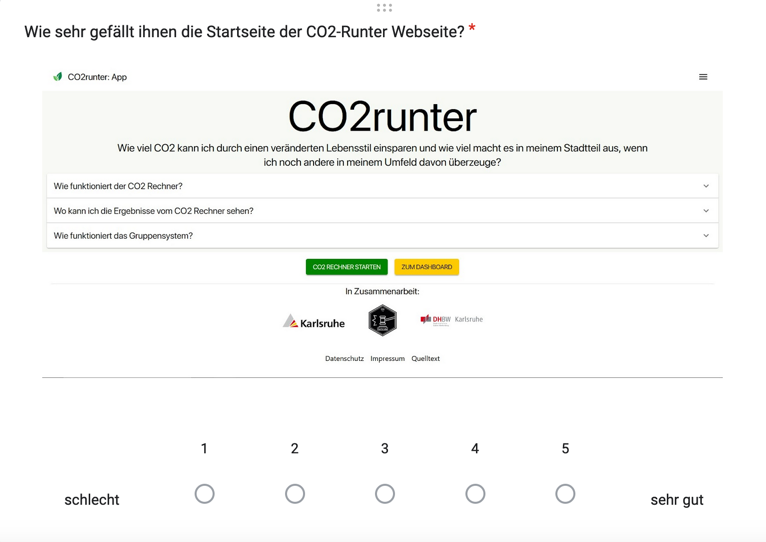
\includegraphics[width=1\textwidth]{images/05/picture_of_evaluation_question}
    \caption{Bewertungsfrage aus Abschnitt 5}
    \label{fig:picture-of-evaluation-question}
\end{figure}

Der andere Fragetyp soll die Meinung der Teilnehmenden zu möglichen neuen Features erfragen.
Dabei wird der Teilnehmer gebeten, eine der folgenden Antwortmöglichkeiten zu nutzen:
Ja, Nein, vielleicht.
Eine beispielhafte Darstellung dieses Fragetyps zeigt Abbildung \ref{fig:picture-of-yes-no-evetually-question}:

Im Anschluss an die erfolgreiche Erstellung der Umfrage wurde diese noch einmal kontrolliert.
Daraufhin wurde sich um eine geeignete Zielgruppe informiert und mit dem Projektteam abgesprochen.
Informationen über den Auswahlvorgang und die angesprochene Personengruppe werden in \hyperref[subsec:auswahl-der-zielgruppe]{Kapitel 4.1.3} (nächste Seite) dokumentiert.
Zu guter Letzt wurde die Umfrage gestartet.

\begin{figure}[H]
    \centering
    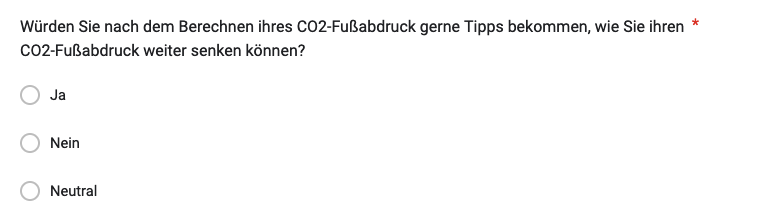
\includegraphics[width=1\textwidth]{images/05/picture_of_yes_no_eventually_question}
    \caption{Ja/Nein/Vielleicht-Frage aus Abschnitt 5}
    \label{fig:picture-of-yes-no-evetually-question}
\end{figure}

\subsection{Fokusdurchführung der Umfrage}

Der Schwerpunkt der Umfrage liegt darin, die Wünsche und Anforderungen der Teilnehmenden zu sammeln, sodass diese im Nachhinein eingearbeitet werden können.
Zu den Wünschen und Schwerpunkten zählen hierbei sowohl Features, die den potenziellen NutzerInnen fehlen und für wichtig erachtet werden.
Zusätzlich sind aber auch Designs und die allgemeine Frage nach dem Design abzufragen und zu sammeln.
Durch die Ergebnisse der Umfrage können dann neue Features eingearbeitet werden, veraltet oder uninteressante Features abgeschafft werden und veraltetes Design überarbeitet werden.
Dadurch kann nach der Durchführung der Implementierung die CO2-Runter Webseite in neuem Glanz erscheinen.

\subsection{Auswahl der Zielgruppe}
\label{subsec:auswahl-der-zielgruppe}

Bevor die Umfrage veröffentlicht wurde, wurde über eine möglichst geeignete Zielgruppe diskutiert.
Im Fokus stand dabei, dass man innerhalb der Zielgruppe möglichst viele Menschen neu für das Thema Klimaschutz gewinnen und überzeugen kann.
Andererseits möchte man mit der Zielgruppe auch erfahrene oder bereits interessierte Menschen ansprechen, sodass man Antworten von Menschen mit Erfahrungen zu diesem Thema erhält.
Dadurch ist zu erwarten, dass sowohl unerfahrene Menschen, als auch Menschen, die sich mit dem Thema Klimaschutz und CO2-Fußabdruck auseinandergesetzt haben, an der Umfrage teilnehmen.

Aus den oben genannten Gründen wurde entschieden, eine Personengruppe mit einer Altersspanne von 12 bis 25 zu wählen.
Diese Zielgruppe verbindet die gewünschten Charateristiken, dass Menschen dieser Personengruppe sowohl Neulinge als auch erfahrene Personen im Bereich Klimaschutz sind.
Zudem ist diese Zielgruppe von Vorteil, da der Klimaschutz und die Reduktion der Ausmaße des Klimawandels ein langjähriger Prozess sein wird.
Dieser Prozess wird vorausschauend hauptsächlich von den jungen Heranwachsenden dieser Zielgruppe getragen.

Um die Zielgruppe möglichst optimal zu treffen, wurde die Umfrage zum größten Teil am Gymnasium Schönau im Schwarzwald durchgeführt.
Den Schülern wurde eine kleine Einführungspräsentation zu der Studienarbeit gegeben.
Anschließend wurde die Umfrage schulweit verbreitet.
Die Umfrage wurde aber auch auf anderen Kommunikationswegen für andere interessierte Personen verbreitet.

\section{Erhebung von Nutzerfeedback}
Die Umfrage wurde am 12. Dezember 2023 veröffentlicht und stand ab diesem Zeitpunkt online zur Verfügung.
Beendet wurde die Umfrage am 22. Februar 2024.
Somit wurde die Befragung zur CO2-Runter Webseite in einem Zeitraum von ungefähr 10 Wochen durchgeführt.
Innerhalb dieses Zeitraums nahmen 67 Personen aktiv an der Umfrage teil.

In diesem Abschnitt sollen einige der Ergebnisse der Befragung präsentiert und offengelegt werden.
Das Feedback und die Antworten der Teilnehmer wird teilweise in Tabellen aufbereitet und nach den Fragekategorien geordnet.
Sollten die Rückmeldungen nicht innerhalb von Tabellen einfach dargestellt werden können, werden die Ergebnisse innerhalb des Fließtextes präsentiert.

Beim ersten Frageabschnitts handelt es sich um den CO2-Fußabdruck.
Innerhalb des Abschnitts wurden fünf Fragen gestellt, die den allgemeinen Wissensstand der Teilnehmer rund um den CO2-Fußabdruck abzufragen.
Vier der fünf Fragen waren sogenannte Ja/Nein-Fragen.
Die Ergebnisse sowie die genau Fragestellung sind in Tabelle \ref{co2fußabdruckfragen} aufgelistet: \newline

\begin{longtable}{|p{0.7\linewidth}|l|l|}
    \hline
    \textbf{Fragestellung}                                                  & \textbf{Ja} & \textbf{Nein} \\ \hline
    \endfirsthead

    Kennen Sie den Begriff CO2-Fußabdruck?                                  & 98,5\%      & 1,5\%         \\ \hline
    Haben Sie sich schon einmal Gedanken über ihren CO2-Fußabdruck gemacht? & 83,6\%      & 16,4\%        \\ \hline
    Haben Sie ihren CO2-Fußabdruck schon einmal berechnet/berechnen lassen? & 58,2\%      & 41,8\%        \\ \hline
    Kennen Sie den Klima-Buddy und haben Sie diesen evtl. schon benutzt?    & 6,0\%       & 94,0\%        \\ \hline
    \caption{Ja/Nein-Fragen aus dem Frageabschnitt CO2-Fußabdruck}
    \label{co2fußabdruckfragen}
    \\
\end{longtable}

Des Weiteren wurde die Frage gestellt, wie bewusst sich die Teilnehmer im Allgemeinen über ihren CO2-Fußabdruck sind.
Als Antwortmöglichkeiten gab es die Zahlen \textit{1} (kein Bewusstsein) bis \textit{5} (volles Bewusstsein).
Insgesamt befinden sich 86,5\% der Befragten im Zahlenraum 2-4.
Lediglich drei der befragten Personen behaupten, vollstes Bewusstsein über ihren CO2-Fußabdruck zu haben.
Auf der anderen Seite besitzen sechs Personen unter den 67 Teilnehmer gar kein Bewusstsein über ihren Fußabdruck.

Im nächsten Frageabschnitt wurde thematisiert, aus welcher Motivation die Teilnehmer die CO2-Runter Webseite benutzen würden.
Insgesamt wurden den Befragten in diesem Abschnitt zehn Fragen gestellt, wovon eine optional war.
Bei vier der neun Pflichtfragen handelt es sich erneut um Ja/Nein-Fragen, die aber eine weitere neutral bzw. unschlüssige Antwortmöglichkeit ermöglichen.
Diese sind mit deren Antwortverteilungen in Tabelle \ref{motivationFragen}aufgelistet:

\begin{longtable}{|p{0.6\linewidth}|l|l|l|}
    \hline
    \multicolumn{1}{|l|}{\textbf{Fragestellung}}                                                   &
    \multicolumn{1}{c|}{\textbf{Ja}}                                                               &
    \multicolumn{1}{c|}{\textbf{Nein}}                                                             &
    \multicolumn{1}{r|}{\textbf{Neutral}}                                                                                     \\ \hline
    \endfirsthead

    Sind Sie bereits aktiv dabei, unser Klima zu schützen?                                         & 61,2\% & 38,8\% & -      \\ \hline
    Motiviert es Sie, wenn Sie ihren Fußabdruck mit anderen Nutzern vergleichen können?            & 56,7\% & 25,4\% & 17,9\% \\ \hline
    Würde ihnen ein Punktesystem helfen, ihren CO2-Fußabdruck häufiger zu berechnen?               & 59,7\% & 19,4\% & 20,9\% \\ \hline
    Würden Sie ihren Fortschritt bzw. ihren CO2-Fußabdruck gerne mit anderen Leuten teilen können? & 26,9\% & 26,9\% & 46,3\% \\ \hline
    \caption{Ja/Nein-Fragen aus dem Frageabschnitt Motivation}
    \label{motivationFragen}
    \\
\end{longtable}

Zusätzlich wurde die folgenden fünf Multiple-Choice-Fragen innerhalb des Motivationsabschnitts gestellt:

\begin{itemize}
    \item \textbf{Warum würden Sie die CO2-Runter Webseite nutzen?}
          \begin{itemize}
              \item aus Interesse (43,4\%)
              \item um mir meinen aktuellen CO2-Fußabdruck berechnen zu lassen (58,2\%)
              \item um Tipps zum Thema Klimaschutz zu erhalten (28,4\%)
              \item aus Neugier (52,2\%)
              \item durch Arbeitskollegen (1,5\%)
          \end{itemize}
    \item \textbf{Was erhoffen Sie sich von einer Webseite, welche den Klimaschutz unterstützt?}
          \begin{itemize}
              \item Aufklärung über den Klimaschutz und den CO2-Fußabdruck (71,6\%)
              \item Tipps, wie ich mein Verhalten zum Schutz unseres Klimas verbessere (73,1\%)
              \item Keinen Vorteil (10,4\%)
              \item Sonstige (3\%)
          \end{itemize}
    \item \textbf{Welche Möglichkeiten müsste eine Webseite ihnen bieten, um unser Klima (noch) aktiver zu schützen?}
          \begin{itemize}
              \item Mehr Tipps, wie ich das Klima schützen kann (38,8\%)
              \item Aufklärung, damit ich sehe wie ich dem Klima schade (61,2\%)
              \item Verlinkung zu Klimaschutzgruppierungen (10,4\%)
              \item Tipps, um den Klimaschutz in den Alltag zu integrieren (80,6\%)
              \item Sonstiges (4,5\%)
          \end{itemize}
    \item \textbf{Welche Anreize könnten Sie dazu motivieren, die Webseite häufiger zu verwenden?}
          \begin{itemize}
              \item Belohnungen (56,7\%)
              \item Wettbewerbe (25,4\%)
              \item soziale Interaktion (23,9\%)
              \item Vergleiche mit anderen (46,3\%)
              \item Keine (3\%)
              \item Sonstiges (6\%)
          \end{itemize}
    \item \textbf{Welche Konzepte finden Sie sinnvoll für eine Webseite, um klimafreundliches Verhalten zu fördern?}
          \begin{itemize}
              \item Gamifizierung (59,4\%)
              \item Soziale Interaktion (31,3\%)
              \item Persönliche Herausforderungen (54,7\%)
              \item Bildung und Bewusstseinsbildung (35,9\%)
              \item Belohnungssystem (53,1\%)
              \item Wettbewerbe (20,3\%)
          \end{itemize}
\end{itemize}

Bei der optionalen Frage wurden die Teilnehmer gebeten, eigene Ideen und Anregungen zu nennen, die sie haben, um klimafreundlicheres Verhalten erzeugen oder unterstützen zu können.
Insgesamt haben neun Personen auf die optionale Frage geantwortet.

Im nächsten Abschnitt wurden den Teilnehmern 13 Fragen zur Nutzerfreundlichkeit der CO2-Runter Webseite gestellt.
Unter den 13 Fragen befinden sich drei optionale Fragen, vier Multiple-Choice-Fragen und sechs Ja/Nein-Fragen.
Die Ja/Nein und die dazugehörigen Ergebnisse sind in Tabelle\ref{nutzerfreundlichkeitFragen} aufgelistet:

\begin{longtable}{|p{0.6\linewidth}|l|l|l|}
    \hline
    \multicolumn{1}{|l|}{\textbf{Fragestellung}}                                                        &
    \multicolumn{1}{c|}{\textbf{Ja}}                                                                    &
    \multicolumn{1}{c|}{\textbf{Nein}}                                                                  &
    \multicolumn{1}{r|}{\textbf{Neutral}}                                                                                          \\ \hline
    \endfirsthead

    Ist ihnen auf dem vorherigen Screenshot der Abschnitt \"Ihr aktueller CO2-Fußabdruck\" aufgefallen? & 46,3\% & 53,7\% & -      \\ \hline
    Wünschen Sie sich, besser durch den            CO2-Rechner geführt zu werden?                       & 23,9\% & 20,9\% & 55,2\% \\ \hline
    Finden Sie es sinnvoll, Zahlenwerte            wie in dieser Abbildung zu schätzen?                 & 44,8\% & 14,9\% & 40,3\% \\ \hline
    Wünschen Sie sich, dass der aktuelle           CO2-Fußabdruck stärker in den Vordergrund rückt?     & 61,2\% & 19,4\% & 19,4\% \\ \hline
    Würden ihnen Richtwerte helfen, die            Kurzantworten besser zu kategorisieren?              & 85,1\% & 4,5\%  & 10,4\% \\ \hline
    Würden Sie die detaillierte Ansicht            bei Fragen nutzen?                                   & 70,1\% & 10,4\% & 19,4\% \\ \hline
    \caption{Ja/Nein-Fragen aus dem Frageabschnitt Nutzerfreundlichkeit}
    \label{nutzerfreundlichkeitFragen}
    \\
\end{longtable}

Bei den Multiple-Choice-Fragen ging es vor allem darum, herauszufinden, welche Aspekte der zu sehenden Webseite besonders nutzerfreundlich und welche eher nicht nutzerfreundlich gestaltet sind.
Dabei wurde sich in der Umfrage auf die Startseite der CO2-Runter Webseite und auf den Fußabdruckrechner fokussiert.
Die Antworten auf die Multiple-Choice-Fragen sind folgendermaßen ausgefallen:

\begin{itemize}
    \item \textbf{Welche Aspekte der aktuellen Startseite finden Sie besonders ansprechend oder benutzerfreundlich?}
          \begin{itemize}
              \item Buttons (47,8\%)
              \item Webseitenbanner (9,0\%)
              \item Infokarten (29,9\%)
              \item Alles (16,4\%)
              \item Gar nichts (19,\%)
          \end{itemize}
    \item \textbf{Welche Aspekte der aktuellen Webseite, welche Sie im Screenshot sehen, finden Sie nicht ansprechend?}
          \begin{itemize}
              \item Buttons (11,9\%)
              \item Webseitenbanner (49,3\%)
              \item Infokarten (19,4\%)
              \item Ich finde alles ansprechend (19,4\%)
              \item Ich finde nichts ansprechend (19,4\%)
              \item Sonstiges (6,0\%)
          \end{itemize}
    \item \textbf{Welche Aspekte des CO2-Rechners finden Sie besonders ansprechend oder benutzerfreundlich?}
          \begin{itemize}
              \item Themenbalken (55,2\%)
              \item Fragebogen (44,8\%)
              \item Anzeige für den aktuellen CO2-Fußabdruck (55,2\%)
              \item Gar nichts (9,0\%)
              \item Sonstiges (3,0\%)
          \end{itemize}
    \item \textbf{Welche Aspekte des CO2-Rechners finden Sie nicht ansprechend?}
          \begin{itemize}
              \item Themenbalken (19,4\%)
              \item Fragebogen (20,9\%)
              \item Anzeige für aktuellen CO2-Fußabdruck (22,4\%)
              \item Ich finde alles prima! (43,3\%)
              \item Farbdesign/Optik (4,5\%)
              \item Sonstiges (3,0\%)
          \end{itemize}
\end{itemize}

Des Weiteren beschäftigen sich drei optionale Fragen mit weiteren Verbesserungsvorschlägen der Teilnehmer.
Pro Frage wurden durchschnittlich 15 Antworten eingereicht.
Im Folgenden sind einige beispielhaft aufgelistet:

\begin{itemize}
    \item \textit{„aktueller CO2 Fußabdruck“ hervorheben } (9x)
    \item \textit{Kennzeichnung durch Farbe} (13x)
    \item \textit{CO2 Fußabdruck Balken farbig hinterlegen}
    \item \textit{Sieht altmodisch aus} (4x)
    \item \textit{Attention-Grabber wie ein Video für die Hauptseite}
    \item \textit{Spielerischere Ansicht, zum erreichen des jüngeren Publikums}
\end{itemize}

Abschließend haben sich die Teilnehmer im letzten Abschnitt mit dem Thema Design befasst.
Im Designabschnitt wird der Teilnehmer dazu aufgefordert, das Design der aktuellen CO2-Runter Webseite zu bewerten.
Zusätzlich werden neue Designvorschläge präsentiert, die ebenfalls bewertet werden sollen.
Innerhalb des Abschnitts werden dem Teilnehmer neun Fragen gestellt.
Davon sind drei Ja/Nein-Fragen, drei Bewertungsfragen, zwei optionale Fragen und ein Designvergleich.
Die Bewertungsfragen befolgen erneut einem Bewertungsschema von den Zahlen \textit{1 bis 5}, wobei 1 die schlechteste Bewertung und 5 die beste Bewertung ist.
Im Folgenden finden Sie die Bewertungsfragen zusammen mit den entsprechenden Antworten:

\begin{itemize}
    \item \textbf{Wie sehr gefällt Ihnen die Startseite der CO2-Runter Webseite?}
          \begin{itemize}
              \item 1, sehr schlecht (20,9\%)
              \item 2, schlecht (19,4\%)
              \item 3, neutral (35,8\%)
              \item 4, gut (19,4\%)
              \item 5, sehr gut (4,5\%)
          \end{itemize}
    \item \textbf{Wie sehr gefällt Ihnen das Design des CO2-Rechners?}
          \begin{itemize}
              \item 1, sehr schlecht (7,5\%)
              \item 2, schlecht (20,9\%)
              \item 3, neutral (44,8\%)
              \item 4, gut (25,4\%)
              \item 5, sehr gut (1,5\%)
          \end{itemize}
    \item \textbf{Wie übersichtlich finden Sie den CO2-Rechner?}
          \begin{itemize}
              \item 1, sehr unübersichtlich (0,0\%)
              \item 2, unübersichtlich (10,4\%)
              \item 3, neutral (31,3\%)
              \item 4, übersichtlich (43,3\%)
              \item 5, sehr übersichtlich (14,9\%)
          \end{itemize}
\end{itemize}

Die Ja/Nein-Fragen und ihre Antworten sind in Tabelle \ref{designFragen} dokumentiert:


\begin{longtable}{|p{0.6\linewidth}|l|l|l|}
    \hline
    \multicolumn{1}{|l|}{\textbf{Fragestellung}}                                                                                                                      &
    \multicolumn{1}{c|}{\textbf{Ja}}                                                                                                                                  &
    \multicolumn{1}{c|}{\textbf{Nein}}                                                                                                                                &
    \multicolumn{1}{r|}{\textbf{Neutral}}                                                                                                                                                        \\ \hline
    \endfirsthead

    Denken Sie, ein FAQ wäre sinnvoll?                                                                                                                                & 71,6\% & 7,5\%  & 20,9   \\ \hline
    Würde eine einfachere Benutzeroberfläche Sie eher                    dazu anregen die Webseite zu nutzen?                                                         & 64,2\% & 10,4\% & 25,4\% \\ \hline
    Würden Sie nach dem Berechnen                                        ihres CO2-Fußabdruck gerne Tipps bekommen,wie Sie ihren CO2-Fußabdruck weiter senken können? & 79,1\% & 3,0\%  & 17,9\% \\ \hline
    \caption{Ja/Nein-Fragen aus dem Frageabschnitt Design}
    \label{designFragen}
    \\
\end{longtable}

Beim Designvergleich wurde das alte Design mit einem Prototyp verglichen.
Laut der Umfrage finden 82,1\% der Befragten den Prototyp besser.
Lediglich 9\% finden das alte Design ansprechender.
Die restlichen 9\% finden weder das alte Design, noch das neue Design besser oder enthalten sich.
Die optionalen Fragen beschäftigen sich erneut mit weiteren Verbesserungsvorschlägen rund um das Design der CO2-Runter Webseite.
Anbei sind einige Antworten der Teilnehmer:

\begin{itemize}
    \item \textit{Cliparts passend zu Thema (Bäume, Weltkugel, Tiere, Menschen, etc.)}
    \item \textit{Moderner gestallten (eyecatcher)}
    \item \textit{Mehr Farbe, mehr Symbole, ansprechendere Schriftart, „jüngeres“ Design}
    \item \textit{Einpflanzung eines Eyecatchers zu dem Thema, wie bei dem bsp. des neuen Designs }
    \item \textit{Mehr Effekte und Farbe, damit es lebhafter wirkt.}
\end{itemize}
\subsection{Erstellung von Personas anhand der Umfrageergebnisse}

Um die Bedürfnisse und Anforderungen der NutzerInnen besser zu verstehen, haben wir die Ergebnisse unserer Umfrage analysiert und Personas erstellt, die typische Nutzergruppen repräsentieren. Dafür ist es typischerweise möglich, diese durch Clustering und andere Methoden zu erstellen. In unserem Fall haben wir uns auf die Analyse der Umfrageergebnisse konzentriert und die Personas basierend auf den Ergebnissen erstellt, weil die Teilnehmeranzahl der Umfrage zu gering war, um eine Clusteranalyse durchzuführen.

Somit haben wir die Umfrageergebnisse analysiert und die wichtigsten Erkenntnisse zusammengefasst. Für die Analyse haben wir die Antworten auf die Fragen zu CO2-Fußabdruck, Motivation, Nutzerfreundlichkeit und Design ausgewertet und durch Mind-Mapping und Brainstorming die wichtigsten Erkenntnisse zusammengefasst. Die Ergebnisse der Umfrage zeigen, dass die Teilnehmer unterschiedliche Kenntnisse und Einstellungen zum Thema Klimaschutz und CO2-Fußabdruck haben.

Zusammenfassend haben wir durch unsere Analyse Personas erstellt, welche typische Nutzergruppen repräsentieren und diese uns helfen, das Verhalten, die Bedürfnisse und die Ziele der Zielgruppe besser zu verstehen. Basierend auf den Ergebnissen unserer Umfrage haben wir die folgenden Personas entwickelt:

\begin{enumerate}
    \item \textbf{Umweltbewusste Person}: Diese Persona ist motiviert, ihren CO2-Fußabdruck zu reduzieren und sich aktiv am Klimaschutz zu beteiligen. Sie ist offen für neue Informationen und Tipps, um ihren Lebensstil nachhaltiger zu gestalten. Diese Persona sucht nach detaillierten Informationen über den Klimawandel und konkreten Anleitungen zur Umsetzung von Maßnahmen.
    \item \textbf{Interessierte Person mit begrenztem Wissen}: Diese Persona ist neugierig darüber, mehr über ihren CO2-Fußabdruck zu erfahren und sucht nach einfachen Möglichkeiten zur Reduzierung. Sie ist offen für neue Ideen und Tipps, benötigt jedoch leicht verständliche Informationen und Anleitungen, um ihren Beitrag zum Klimaschutz zu leisten.

    \item \textbf{Skeptische Person}: Diese Persona steht dem Thema Klimaschutz skeptisch gegenüber und benötigt fundierte Informationen und Beweise, bevor sie ihr Verhalten ändert. Sie ist nicht bereit, große Veränderungen im Lebensstil vorzunehmen, und sucht nach praktischen Möglichkeiten zur Reduzierung ihres CO2-Fußabdrucks, ohne bevormundet zu werden.
\end{enumerate}

% Überleitung ins nächste Kapitel

Durch die Konzentration auf diese Personas und das Verständnis ihrer Bedürfnisse und Motivationen ist es uns möglich geworden, die Webseite aus der Perspektive der NutzerInnen zu betrachten und die Benutzererfahrung zu verbessern. Dadurch konnten wir spezifische Anforderungen definieren und die Webseite so gestalten, dass sie die Bedürfnisse und Ziele der Zielgruppe besser erfüllt.
Die Anforderungen werden im nächsten Kapitel vorgestellt und behandelt.
Es wird erklärt, welche Art von Anforderungen definiert wurden und wie die konkreten Anforderungen aussehen.

% \subsection{Analyse der Umfrageergebnisse}

